\documentclass[11pt,a4paper]{article}
\usepackage[utf8]{inputenc}
\usepackage[british]{babel}
\usepackage[a4paper,margin=2.3cm]{geometry}
\usepackage{amsmath,amssymb}
\usepackage{graphicx}
\usepackage{tikz}
\usetikzlibrary{calc,angles,quotes,patterns}
\usepackage[most]{tcolorbox}
\usepackage{enumitem}
\usepackage{array}
\usepackage{titlesec}
\usepackage[hidelinks]{hyperref}

\definecolor{bandgreen}{RGB}{46,139,87}
\definecolor{bandblue}{RGB}{30,100,190}
\definecolor{bandamber}{RGB}{220,140,20}
\definecolor{bandpink}{RGB}{210,70,140}
\definecolor{bandpurple}{RGB}{110,50,160}

\newcounter{prob}
% \prob{label}{title}{source}
\newcommand{\prob}[3]{\par\bigskip\refstepcounter{prob}\label{#1}%
  \noindent\textbf{\theprob.\ #2}\hfill{\small\textit{#3}}\par\nopagebreak\smallskip}
\newcommand{\ans}[2]{\par\smallskip\noindent\textbf{\ref{#1}.}\ #2}

\newcommand{\band}[3]{%
  \clearpage
  \begin{tcolorbox}[colback=#1!12,colframe=#1,boxrule=1pt,arc=2pt]
  {\Large\bfseries\color{#1} #2}\hfill{\large #3}
  \end{tcolorbox}}

\newtcolorbox{diarynote}[1]{colback=black!4,colframe=black!45,boxrule=0.6pt,
  arc=2pt,fonttitle=\bfseries\small,title={#1},fontupper=\small}

\setlength{\parindent}{0pt}
\setlength{\parskip}{3pt}
\begin{document}

\begin{titlepage}
\centering
\vspace*{2cm}
{\Huge\bfseries The Ladies' Diary\par}
\vspace{0.6cm}
{\Large One hundred and two problems, 1707--1748,\\ for readers from five to seventeen\par}
\vspace{1.2cm}
\includegraphics[width=0.62\textwidth]{diary_p1.jpg}\par
\vspace{0.4cm}
{\small The first page of mathematical questions in Thomas Leybourn's
\textit{The Mathematical Questions, Proposed in the Ladies' Diary, and Their Original
Answers}, vol.~I (London, 1817), p.~1. Scan: Google Books, via the Internet Archive.\par}
\vfill
{\large Working draft\par}
\end{titlepage}

\section*{A word before the problems}

In 1704 John Tipper, a Coventry schoolmaster, began an almanac for women. It had the
usual things an almanac has. It also had riddles. Within a few
years the riddles had turned into arithmetic, and the arithmetic into geometry. By the
time Tipper stepped down in 1713 his readers were setting each other problems that
would not disgrace a university.\footnote{Leybourn, \textit{Mathematical Questions},
vol.~I, preface, pp.~viii--ix. The Diary ran until 1840, when it merged with its rival,
the \textit{Gentleman's Diary}; the last issue bore the date 1841, which is why some
sources give that year. See J.~Albree and S.~H.~Brown, `A valuable monument of
mathematical genius': The Ladies' Diary (1704--1840), \textit{Historia Mathematica} 36
(2009).}

Many of the people who answered were women. Mary Wright answered the prize question
for 1709. Barbara Sidway set problems as well as solving them; one of hers, the largest
cylinder that can be cut from a cone, is problem~\ref{u-sidway} in this booklet. Lydia
Fisher and Sarah Brown set questions too. Anna Wright set the prize question for 1713:
which bright star stood nearest the north pole at the Creation, taken to be 5,716 years
earlier? It is astronomy, so it is not in this booklet. John Edens answered it: the
third star of Draco, counted from the tip of the tail.\footnote{Leybourn,
\textit{Mathematical Questions}, vol.~I, p.~35.} The Diary asked for no qualifications. It
asked for an answer, and printed the best one.

This booklet takes one hundred and two of those problems and sorts them by age. The
source is the first volume of Thomas Leybourn's collection of 1817, which gathers the
mathematical questions from 1707 to 1748 with their original answers. Nothing here needs
physics or an almanac: questions about pendulums, falling bodies, sound, the sun's
declination and the like have been left out.

\subsection*{How to read the labels}

Each problem carries its source. \textit{Q23} means question~23 in Leybourn's
volume~I, printed as the Diary printed it, in modern words. \textit{After Q23} means
the problem has been retold: new numbers for young readers, or modern money and metres
in place of groats, nobles and chains. The idea is always the Diary's. Where a retelling
changes the answer, the answer given is for the retelling.

Leybourn's own numbering has two slips. There are two questions numbered~2 (the age
rhyme and the garden walk) and two numbered~131 (the pair of series and the Molten Sea).
They are cited here as \textit{Q2 (second)} and \textit{Q131 (second)}.

\subsection*{The bands}

\begin{center}
\begin{tabular}{>{\bfseries}l l l r}
\color{bandgreen}Green  & ages 5--8   & counting, halving, doubling          & 6\\
\color{bandblue}Blue    & ages 8--11  & arithmetic, first patterns          & 6\\
\color{bandamber}Amber  & ages 11--14 & ratio, fractions, first algebra     & 29\\
\color{bandpink}Pink    & ages 14--16 & GCSE: quadratics, Pythagoras, volume & 40\\
\color{bandpurple}Purple & ages 16--17 & A-level: calculus, series, proof    & 21\\
\end{tabular}
\end{center}

Answers are at the back. Some of them are not the Diary's: the Diary was sometimes
wrong, and when it was, a small grey box says so.
\subsection*{How this edition was made}
This edition was prepared with the assistance of Claude, an AI model made by Anthropic. Under the editor's direction, Claude drafted the retellings, solutions, notes and introduction, recomputed every answer, ran optical character recognition on the source scans (using Tesseract) to check names and dates, and typeset the text. Selection, editorial decisions and final responsibility for the text are the editor's.

%================ GREEN ================
\band{bandgreen}{Green}{ages 5--8}

\prob{g1}{Counting the treasure}{after Q1}
A shopkeeper counts his coins, 10 every minute. How many minutes does he need to count
100 coins?

\prob{g2}{The merchant's boxes}{after Q6}
A merchant sells a king five boxes. For the first box he asks 1 grain of wheat, for the
second 2 grains, for the third 4, and each time twice as many as before. How many grains
for the fifth box? How many for all five together?

\prob{g3}{Sharing the sweets}{after Q23}
Share 7 sweets between a mother, a daughter and a son. Mother must have twice as many as
her daughter, and the son twice as many as his mother.

\prob{g4}{Changing places}{after Q37}
Three friends, Ann, Ben and Cara, have dinner together every day. Each day they sit in a
different order on the bench. How many days can they do this before they must repeat an
order?

\prob{g5}{Voting for the class pet}{after Q107}
A class votes for its pet: 18 votes altogether. The cat gets 2 more votes than the dog,
and 4 more than the rabbit. How many votes does each pet get?

\prob{g6}{The little magic square}{after Q126}
Put the numbers 1, 3, 7 and 9 in the empty boxes so that every row, every column and
both diagonals add up to 15.
\begin{center}
\renewcommand{\arraystretch}{1.8}
\begin{tabular}{|>{\centering\arraybackslash}p{0.9cm}|>{\centering\arraybackslash}p{0.9cm}|>{\centering\arraybackslash}p{0.9cm}|}
\hline 4 & & 2\\ \hline & 5 & \\ \hline 8 & & 6\\ \hline
\end{tabular}
\end{center}

%================ BLUE ================
\band{bandblue}{Blue}{ages 8--11}

\prob{b1}{A million million pounds}{Q1}
How long would it take to count a million million pounds, counting £100 every minute
without a break? Take a year as 365 days, 5 hours and 45 minutes. A calculator will
help.

\prob{b2}{The Indian merchant's diamonds}{Q6}
A merchant offers the King of Persia sixty-four diamonds. For the first he asks one grain
of wheat, for the second two, for the third four, doubling each time. The king thinks a
few sacks of wheat will pay for the lot.
\begin{enumerate}[label=(\alph*),nosep]
\item How many grains for the tenth diamond?
\item Add up the grains for the first 1, 2, 3, 4 and 5 diamonds. What do you notice?
\item Use what you noticed to say how many grains the king owes for all sixty-four.
Was he right about the sacks?
\end{enumerate}

\prob{b3}{The will and the twins}{Q23}
A man dies leaving £7,000 and a wife expecting a child. His will says: if the child is a
son, the mother gets one-third and the son the rest; if a daughter, the mother gets
two-thirds and the daughter the rest. The mother has twins, a son and a daughter. How
should the money be shared so as to keep to what the father wanted?

\prob{b4}{Nine at dinner}{Q37, by John Hodge of Truro}
Nine friends agree to put off an unpleasant job for as many days as they can sit down
to dinner in a different order. How long can they put it off?

\prob{b5}{The election}{Q107}
Four candidates stand for election and 5,219 votes are cast. The winner has 22 more
votes than the second, 73 more than the third and 130 more than the fourth. How many
votes does each receive?

\prob{b6}{The magic square of sixteen}{Q126, by Thomas Dodd}
Place the sixteen numbers
\[8,\ 9,\ 10,\ 11,\ 14,\ 15,\ 16,\ 17,\ 20,\ 21,\ 22,\ 23,\ 26,\ 27,\ 28,\ 29\]
in a four-by-four square so that every row, every column and both diagonals add up
to~74.
%================ AMBER ================
\band{bandamber}{Amber}{ages 11--14}

\prob{a-rhyme}{The age rhyme}{Q2}
\begin{quote}\itshape
If to my age there added be\\
One half, one third, and three times three;\\
Six score and ten the sum you'd see,\\
Pray find out what my age may be.
\end{quote}
(A score is twenty.)

\prob{a-wine}{The wine merchant}{after Q3}
A merchant pays £19 for 13 barrels of wine. Each barrel holds 150 litres. How many
litres can he buy for £95?

\prob{a-hay}{The hay bill}{after Q4}
A farmer pays £178 for 15 loads of hay. How much will 90 loads cost? He pays part of the
bill with sixteen £20 notes and the rest in £1 coins. How many coins does he need?

\prob{a-wedding}{The wedding day}{Q5}
On his wedding day a man noticed that he was three times as old as his wife. Fifteen
years later he was only twice as old. How old were they on the wedding day?

\prob{a-coins}{Three kinds of coin}{after Q11}
A man has only £2 coins, £1 coins and 50p coins. His £1 and 50p coins together number
409, and his £1 and £2 coins together number 1,254. If 42 coins were taken from his £2
and 50p coins together, 1,103 would remain. How many coins of each kind does he have,
and how much money is that?

\prob{a-servant}{The idle servant}{after Q13}
A farmer hires a servant for 27 days. For every day he works he earns £16, and for every
day he is idle he is fined £20. At the end neither owes the other anything. How many
days did he work?

\prob{a-spark}{The impertinent young man}{Q15}
A lady, asked her age by an impertinent young man, replied: ``Multiply my age by three.
Take two-sevenths of that and treble it. The square root of two-ninths of the result
is four. Now tell me my age, or never see me again.'' How old was she?

\prob{a-fisher}{Lydia Fisher's numbers}{Q18, by Lydia Fisher}
Find two numbers whose sum is $16\tfrac12$ and such that the greater divided by the
less gives~27.

\prob{a-shepherd}{The shepherdesses}{Q21, by Gideon Cosier}
A gentleman riding past a common asks some shepherdesses how many sheep they have. One
answers: ``If the flock were shared equally among us, each would have twice as many
sheep as there are shepherdesses. But if one of us had 1 sheep, the next 2, the next 4,
and so on, doubling each time, the last would have as many sheep as there are in the
whole flock.'' How many shepherdesses, and how many sheep?

\prob{a-months}{An age in months}{Q27, by John Wilson}
A man says: ``Add to the number of months in my age one half and one eighth of it, and
the sum is 442.'' How old is he?

\prob{a-brown}{The patient lover}{Q29, by Sarah Brown}
A young woman tells her suitor she will marry him when the square of her age, less
one-ninth of itself and then increased by one-third of itself, comes to 891. How old
will she be?

\prob{a-army}{The army on the plain}{after Q34}
An army of 60,000 soldiers stands in a rectangle whose sides are in the ratio $3:2$, with
2 metres between neighbours. How much ground does it cover?

\prob{a-estate}{The father's estate}{Q35, by John Wilson}
A father tells his daughter's suitor that the cube of the number of pounds in his estate
is $352947\times64\times9$, and that he will give three-sevenths of it as her marriage
portion. He will not consent to the match until the young man says what the portion is.
What is it?

\prob{a-names}{The old man's name}{Q43, by Mrs Boydell}
\begin{quote}\itshape
An aged sire, with his two daughters, came\\
To town, and was desir'd to tell his name.\\
My name, says he, 's a thousand more than you\\
And I; and if you add the other two,\\
The number of this present year they'll shew.\\
The num'ral letters of our names (well set\\
With the first letter of the alphabet)\\
Make seventeen hundred, and fourteen complete.\\
I'll further add (to make the problem plain)\\
Each single name five letters doth contain.
\end{quote}
Find the three names. (Read the Roman numerals in each name: D is 500, C 100, L 50,
V or U 5, I 1. The year was 1714.)

\prob{a-walnut}{The walnut trees}{Q48}
A garden is surrounded by walnut trees which gave 2,187 walnuts one season. Each tree had
as many branches as there were trees, and each branch bore 3 walnuts. How many trees?

\prob{a-legacy}{The legacy}{after Q55, by Xantippe}
M, A and N share a legacy of £6,600. Whenever M receives £3, A receives £2; whenever A
receives £5, N receives £4. What does each receive?

\prob{a-magic10}{The great magic square}{Q61, by Peter Ward}
Place the numbers 1 to 100 in a ten-by-ten square so that every row, every column and
both diagonals add up to~505.

\prob{a-gold}{The gold block}{after Q65}
A block of gold is a cuboid. Its length times its depth is 96\,cm$^2$, its breadth
times its depth is 80\,cm$^2$, and its length times its breadth is 120\,cm$^2$. What are
its dimensions and volume?

\prob{a-lcm}{Divisible by every digit}{Q73}
Find the least number that can be divided by each of the numbers 1 to 9 without a
remainder. Then give a rule for finding the least number divisible by any given
numbers.

\prob{a-world}{Round the world}{after Q83}
Two travellers leave Bristol at the same time. One walks round a circle of latitude,
13,500\,km long, at 30\,km a day. The other walks round a circle through the poles,
40,000\,km long, at 50\,km a day. After how many days are both back at Bristol together,
and how many times has each gone round?

\prob{a-fares}{The passengers' fares}{after Q89, by Adrastea}
Twenty-four people, some captains, some mates, some sailors and some boys, pay £48 for a
passage. A captain pays £8, a mate £4, a sailor £1 and a boy 50p. There is at least one
of each. How many of each could there be? Find every way.

\prob{a-labourer}{The labourer's year}{after Q144}
A labourer is hired for a year of 365 days. He earns £70 for each day he works and is
fined £30 for each day he is idle. At the end of the year his fines exactly cancel his
earnings. How many days did he work?

\prob{a-aliquot}{Each made of the other's parts}{Q162, by Christopher Mason}
The aliquot parts of a number are its divisors other than itself: those of 12 are 1, 2,
3, 4 and 6. Find two numbers $A$ and $B$ such that the aliquot parts of $A$ add up to
two-thirds of $B$, and the aliquot parts of $B$ add up to three-quarters of $A$.

\prob{a-perfect}{Perfect numbers}{Q166, by Christopher Mason}
A number is perfect if its aliquot parts add up to the number itself, as
$6 = 1 + 2 + 3$. Give a rule that produces perfect numbers, and use it to find all the
perfect numbers below ten million.

\prob{a-field}{The larger field}{after Q176}
A rectangular field would be 64\,m$^2$ larger if it were 2\,m wider and 3\,m longer. It
would be 68\,m$^2$ larger if it were 3\,m wider and 2\,m longer. What are its dimensions
and area?

\prob{a-battalion}{The square battalion}{Q183, by Thomas Fearn}
A general draws up his army in a square and finds 284 soldiers left over. He adds one
man to each side of the square and finds he is 25 short. How many soldiers has he?

\prob{a-birthday}{A birthday in proportion}{Q184, by Eumenes Pamphilus}
Three numbers are in continued proportion: the first is to the second as the second is
to the third. Their product is 512 and the two outer numbers add up to 34. Take
three-quarters of the greatest as years and the other quarter as weeks: that is my age.
The middle number is the month and the least the day of the month on which I was born.
Find the numbers and my birthday.

\prob{a-billiards}{The six-sided billiard table}{Q215, by John May of Amsterdam}
A billiard table has six straight cushions. Ball $A$ is to be struck so that it bounces
off each cushion in turn, going round the table, and then hits ball $B$. Show how to find
with ruler and compasses the points where it must strike the cushions. Treat the balls
as points, and assume each bounce makes equal angles with the cushion.
\begin{center}
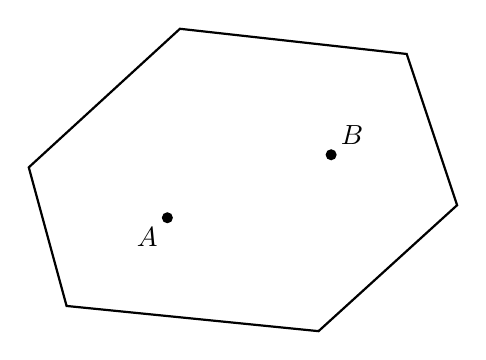
\begin{tikzpicture}[scale=0.8]
\draw[thick] (0,0)--(4,-0.4)--(6.2,1.6)--(5.4,4)--(1.8,4.4)--(-0.6,2.2)--cycle;
\fill (1.6,1.4) circle (2.5pt) node[below left]{$A$};
\fill (4.2,2.4) circle (2.5pt) node[above right]{$B$};
\end{tikzpicture}
\end{center}

\prob{a-clock}{Hands in a line}{Q255}
Looking at a distant clock, I could not read the figures, but I could see that the
minute hand pointed up and to the right while the hour hand pointed down and to the left,
the two making one straight line tilted about $50^\circ$ above the horizontal. What time
was it?
%================ PINK ================
\band{bandpink}{Pink}{ages 14--16}

\prob{p-garden}{The garden walk}{Q2 (second)}
A gentleman has a rectangular garden 100\,m long and 80\,m wide. He wants a path of equal
width running half way round it, along one long side and one short side, that will take
up exactly half the garden. How wide must the path be?
\begin{center}
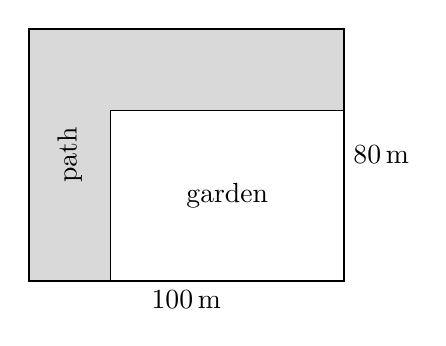
\begin{tikzpicture}[scale=0.04]
\fill[black!15] (0,0) rectangle (100,80);
\fill[white] (26,0) rectangle (100,54);
\draw[thick] (0,0) rectangle (100,80);
\draw (26,0)--(26,54)--(100,54);
\node at (63,27) {garden};
\node[rotate=90] at (13,40) {path};
\node[below] at (50,0) {100\,m}; \node[right] at (100,40) {80\,m};
\end{tikzpicture}
\end{center}

\prob{p-fathers}{Two fathers and a son}{Q7}
Two men of the same age are talking. One says: ``My eldest son is exactly half my age,
and if 340\,\textonehalf{} is added to the product of our three ages, the total is 30,000.''
Find the three ages.

\prob{p-vintner}{The vintner's mixture}{after Q8}
A wine seller has wines at £32, £20 and £16 a bottle. He wants to make up 56 bottles
worth £22 a bottle on average, using whole bottles of each kind. In how many ways can he
do it?

\prob{p-grind}{The grindstone}{Q9}
Seven people buy a grindstone 60\,cm across and agree that each will use it in turn
until they have ground away exactly one-seventh of it. How much of the diameter does
each grind away?
\begin{center}
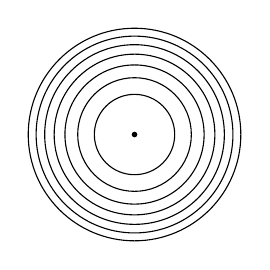
\begin{tikzpicture}[scale=0.045]
\foreach \k in {7,6,5,4,3,2,1} \draw ({0},{0}) circle ({30*sqrt(\k/7)});
\fill (0,0) circle (0.8);
\end{tikzpicture}
\end{center}

\prob{p-tether}{The tethered horse}{after Q14}
How long must a horse's tether be for it to graze exactly 1,000\,m$^2$?

\prob{p-kettle}{The tinker's kettle}{after Q17, answered by Richard Parker}
\begin{quote}\itshape\small
I happen'd one ev'ning with a tinker to sit,\\
Whose tongue ran a great deal too fast for his wit:\\
He talk'd of his art with abundance of mettle,\\
So I ask'd him to make me a flat-bottom kettle,\\
That the top and the bottom diameters be\\
In just such proportion as five is to three.\\
Twelve inches the depth I would have, and no more,\\
And to hold in ale gallons seven less than a score.\\
He promis'd to do't, and to work he strait went;\\
But when he had done it, he found it too scant.\\
He alter'd it then, and too big he had made it,\\
And when it held right, the diameters fail'd it:\\
So that making it often, too big or too little,\\
The tinker at last had quite spoil'd the kettle:\\
Yet he vows he will bring his said purpose to pass,\\
Or he'll utterly spoil ev'ry ounce of his brass.\\
To prevent him from ruin, I pray help him out,\\
The diameter's length else he'll never find out.
\end{quote}
In modern measures: the kettle is a frustum of a cone, 30\,cm deep, holding 50 litres,
with top and bottom diameters in the ratio $5:3$. Find the diameters.

\prob{p-fractions}{Two fractions}{Q19}
Find two fractions whose sum is $\tfrac17$ and whose product is $\tfrac{4}{847}$.

\prob{p-ship}{North, then west}{Q22, by Amos Fish}
A ship sails due north for some distance, then due west. The westward run is 60 miles
longer than the northward one. The perpendicular from the turning point to the straight
line joining the ship to its port is 150 miles. How far did it sail, and how far is it
from port? (Treat the sea as flat.)

\prob{p-bushel}{The bushel measure}{after Q26}
A cylindrical measure is 20\,cm deep and 46\,cm across. Another measure must hold the
same amount but be only 18\,cm deep. How wide must it be?

\prob{p-ladder}{The ladder}{Q31, by Robert Wilson}
A ladder 100\,m long stands upright against a wall 100\,m high. How far does the top slide
down if the foot is pulled out 10\,m from the wall?
\begin{center}
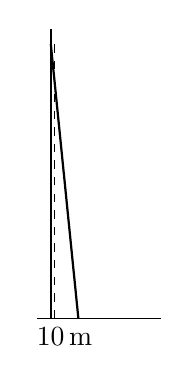
\begin{tikzpicture}[scale=0.035]
\draw[thick] (0,0)--(0,105); \draw (-5,0)--(40,0);
\draw[dashed] (1.5,0)--(1.5,100);
\draw[thick] (10,0)--(0,99.5);
\node[below] at (5,0) {10\,m};
\end{tikzpicture}
\end{center}

\prob{p-tippler}{The tippler}{after Q41}
Asked how much he had spent, a man replied: ``Square the number of pounds, multiply by
five times its square root, and you get 38,880.'' How much did he spend?

\prob{p-maypole}{The maypole}{Q42, by William Taylor}
A wind snaps a maypole. The broken part is 63\,m long and its top strikes the ground
30\,m from the foot of the pole. How tall was the maypole?
\begin{center}
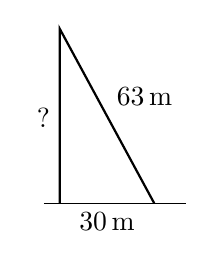
\begin{tikzpicture}[scale=0.04]
\draw (-5,0)--(40,0); \draw[thick] (0,0)--(0,55.4)--(30,0);
\node[left] at (0,27) {?}; \node[below] at (15,0) {30\,m};
\node[above right] at (15,28) {63\,m};
\end{tikzpicture}
\end{center}

\prob{p-head}{Head and feet}{after Q45, by Thomas Shepheard}
A person 1.5\,m tall walks 10,000\,km round the Earth along a great circle. Taking the
Earth's circumference as 40,000\,km, how much farther does their head travel than their
feet?

\prob{p-ap}{Four in progression}{Q49, by William Hawney}
Find four numbers in arithmetic progression with common difference 4 whose product is
176,985.

\prob{p-sons}{Two sons}{Q58, by Lady Mer.~Heyshot}
A lady observes that if her younger son's age is taken from the square of her elder
son's age, the remainder is 425; and if the elder's age is taken from the square of the
younger's, the remainder is 235. How old are they?

\prob{p-decagon}{The decagon}{Q59}
Find the side of a regular decagon whose area is 169\,m$^2$.

\prob{p-pond}{The broken pole}{after Q60, by Thomas Gary of Lynn}
A pole 100\,m high stands in the middle of a circular pond whose area is
$1600\pi$\,m$^2$. The pole snaps and its top just reaches the edge of the pond. How tall
is the part left standing?
\begin{center}
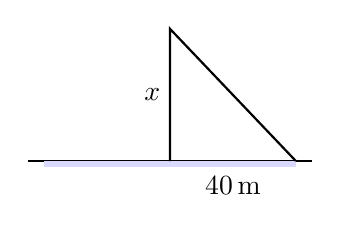
\begin{tikzpicture}[scale=0.04]
\draw (-45,0)--(45,0); \fill[blue!15] (-40,-2) rectangle (40,0);
\draw[thick] (0,0)--(0,42)--(40,0);
\node[left] at (0,21) {$x$}; \node[below] at (20,-2) {40\,m};
\end{tikzpicture}
\end{center}

\prob{p-chords}{Two chords}{Q68}
A chord of a circle is 60\,m long and its height above the arc (the versed sine) is
10\,m. In the same circle, what is the height of the segment whose chord is 90\,m?

\prob{p-field}{The triangular field}{after Q70}
Two sides of a field meet at an angle of $30^\circ$, and their product is
16,000\,m$^2$. Find the area of the field.

\prob{p-prize}{The prize money}{Q72, by Mary Nelson}
A captain shares prize money among his crew. The first man takes £1 and one-hundredth of
what remains; the second £2 and one-hundredth of what then remains; the third £3 and
one-hundredth of the rest; and so on, the last taking all that is left. It turns out
that everyone receives the same. How many men were there, and how much did each get?

\prob{p-earth}{Filling the hollow Earth}{after Q80}
Suppose the Earth were a hollow sphere with a circumference of 40,000\,km, and a river
12\,m wide and 6\,m deep flowed into it at 1\,km an hour. How many years would it take
to fill?

\prob{p-house}{The house}{Q81, by J. Jennings}
The cost of building a house exceeded the builder's profit on it by £160, and the squares
of the cost and the profit add up to 70,600. Find the cost and the profit, in pounds.

\prob{p-temples}{Two temples}{Q84, by Samuel Dicker}
Two square temples are paved with tiles one metre square, 2,120 tiles in all. Each side of
one floor is 12\,m longer than each side of the other. Find the sides.

\prob{p-extreme}{Extreme and mean}{Q90}
A father leaves £50,000 to his two sons so that the square of the elder's share equals
50,000 times the younger's share. What does each receive?

\prob{p-tub}{The tub}{after Q95, by Alexander Naughley}
A tub is a frustum of a cone with its bottom diameter 32\,cm. Its two diagonals cross,
cutting each other into pieces of 20\,cm (below) and 30\,cm (above). Find the volume.
\begin{center}
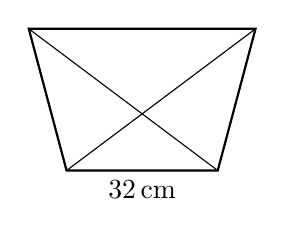
\begin{tikzpicture}[scale=0.06]
\draw[thick] (-16,0)--(16,0)--(24,30)--(-24,30)--cycle;
\draw (-16,0)--(24,30); \draw (16,0)--(-24,30);
\node[below] at (0,0) {32\,cm};
\end{tikzpicture}
\end{center}

\prob{p-southsea}{The South Sea losses}{Q98, by T. Rasberry}
Three people lost money in the South Sea Bubble. A lost £2,000 more than B and £9,000
more than C, and the square of A's loss equals the sum of the squares of the other two.
What did each lose?

\prob{p-moat}{The tower across the moat}{Q105}
A moat round a tower is 93\,m wide. If the height of the tower is multiplied by 93 and
twice the length of a ladder reaching from the outer edge of the moat to the top is
added, the total is 14,423. How high is the tower?

\prob{p-golden}{The golden field}{after Q116}
A rectangular field's perimeter plus its diagonal comes to 800\,m. A line equal to the
diagonal plus the shorter side, divided in extreme and mean ratio, has the diagonal as
its larger part. Find the sides, and the cost of turfing the field at £2 a square metre.

\prob{p-quotients}{Parts and quotients}{Q118}
Divide 10,000 into two parts such that when each is divided by the other, the two
quotients add up to~5.

\prob{p-close}{The rectangular close}{Q122, by Samuel Marriot}
A rectangular field has lost its fences. The owner remembers that a perpendicular drawn
from one corner to a diagonal cut off 16\,m of that diagonal, and that the same
perpendicular, extended 2\,m beyond the diagonal, met the far long side. The diagonal and
the extended perpendicular are to divide the field into four shares for his
grandchildren. Find the shares.

\prob{p-molten}{The Molten Sea}{Q131 (second), by John Hartley}
Solomon's Molten Sea was a bronze cylinder holding 2,000 baths. A line of 30 cubits went
round the outside, the inside was 5 cubits deep, and the metal was a hand's breadth
thick. Taking a cubit as 55.6\,cm and a hand's breadth as 9.27\,cm, how many litres
were in a bath?

\prob{p-york}{Messengers to York}{Q136}
London and York are 150 miles apart, and Stilton divides the road in extreme and mean
ratio, the longer part being from Stilton to York. Two messengers leave London together,
each travelling steadily, one to Stilton and one to York, and they arrive at the same
moment. Compare their speeds.

\prob{p-eclipse}{The eclipse triangle}{Q147, by Thomas Williams}
In a right-angled triangle the base and the perpendicular together make 83, and the base
and the hypotenuse together make 116. Find the three sides.

\prob{p-speidel}{The square in the triangle}{Q153, by George Anderson}
In triangle $ABC$, let $BP$ be the perpendicular from $B$ to the base $CA$. At $C$ erect
$CD$ perpendicular to $CA$, equal to $BP$ and on the same side as $B$, and join $DA$. Let
the line bisecting angle $ACD$ meet $DA$ at $N$. Prove that the line through $N$ parallel
to $CA$ cuts $BC$ and $BA$ at points $G$ and $H$ such that $GH$ is the side of the square
standing on $CA$ inside the triangle. (John Speidel gave this construction in 1617.)
\begin{center}
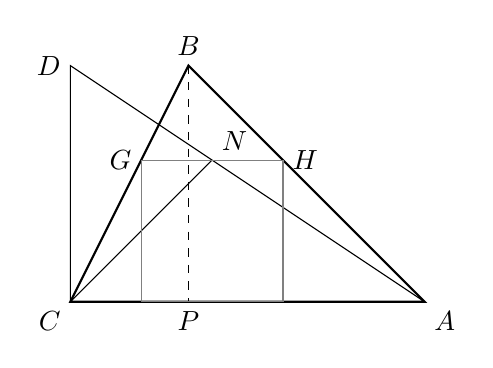
\begin{tikzpicture}[scale=0.75]
\coordinate (C) at (0,0); \coordinate (A) at (6,0); \coordinate (B) at (2,4);
\coordinate (P) at (2,0); \coordinate (D) at (0,4);
\draw[thick] (C)--(A)--(B)--cycle; \draw[dashed] (B)--(P);
\draw (C)--(D)--(A); \draw (C)--(2.4,2.4);
\coordinate (N) at (2.4,2.4);
\draw (1.2,2.4)--(3.6,2.4);
\draw[black!50] (1.2,0) rectangle (3.6,2.4);
\foreach \p/\l in {C/below left,A/below right,B/above,P/below,D/left,N/above right}
  \node[\l] at (\p) {$\p$};
\node[left] at (1.2,2.4) {$G$}; \node[right] at (3.6,2.4) {$H$};
\end{tikzpicture}
\end{center}

\prob{p-legs}{Squares on the legs}{Q170, by Samuel Ashby}
Triangle $ABC$ is right-angled at $B$. Squares are drawn outwards on $AB$ and $BC$; let
$D$ be the corner of the square on $AB$ opposite $B$, and $E$ the corner of the square on
$BC$ opposite $B$. Line $DC$ cuts $AB$ at $F$ and line $EA$ cuts $BC$ at $G$. Prove that
$BF = BG$, and that each is a mean proportional between $AF$ and $CG$.
\begin{center}
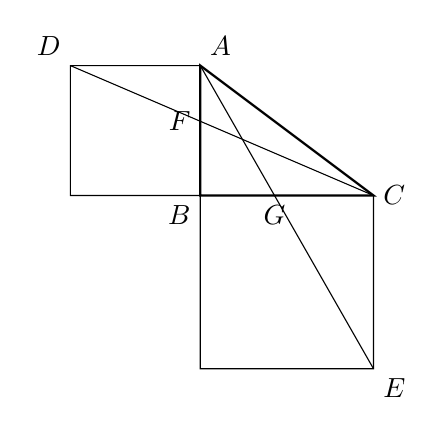
\begin{tikzpicture}[scale=0.55]
\coordinate (B) at (0,0); \coordinate (A) at (0,3); \coordinate (C) at (4,0);
\coordinate (D) at (-3,3); \coordinate (E) at (4,-4);
\draw[thick] (A)--(B)--(C)--cycle;
\draw (B)--(-3,0)--(D)--(A); \draw (C)--(E)--(0,-4)--(B);
\draw (D)--(C); \draw (E)--(A);
\coordinate (F) at (0,{12/7}); \coordinate (G) at ({12/7},0);
\foreach \p/\l in {A/above right,B/below left,C/right,D/above left,E/below right,F/left,G/below}
  \node[\l] at (\p) {$\p$};
\end{tikzpicture}
\end{center}

\prob{p-steeple}{The steeple}{after Q172, by Christopher Hale}
Two lines whose product is 1,800\,m$^2$ form two sides of a triangle, and the triangle's
area is as large as possible. The third side equals the height of a steeple. How tall
is the steeple?

\prob{p-manors}{The four manors}{Q180, by John Gundy}
A gentleman owns four manors whose areas in hectares are in continued proportion. The two
middle areas add up to 1,152 and the two outer ones to 1,728. Find the four areas.

\prob{p-stone}{The stone in progression}{Q191, by John Turner}
A block of stone is a cuboid whose depth, breadth and length are in arithmetic
progression. Its volume is 5,184\,cm$^3$, and the common difference is one forty-eighth
of the length times the depth. Find the dimensions.

\prob{p-pigs}{The Dutch pigs}{after Q207, by John May of Amsterdam}
Three couples buy pigs at market. Each person pays as many pounds for each pig as the
number of pigs they buy, and each husband spends £63 more than his wife. Hendrick buys 23
more pigs than Catriin, and Claas buys 11 more than Geertruii. The wives are Geertruii,
Catriin and Anna, the husbands Hendrick, Claas and Cornelius. Who is married to whom?

\prob{p-firs}{Two firs and a fountain}{prize question, 1711}
In a level garden stand two firs, 100\,m and 80\,m tall, their feet 120\,m apart, each
with a gilt ball on top. The owner wants a fountain on the line between their feet,
equally distant from the two balls; a straight walk from the fountain, every point of
which is equally distant from the two balls; and at the end of the walk a summer-house,
where a couch is as far from each ball as the balls are from each other. Where do the
fountain and the summer-house go, and how long is the walk?
%================ PURPLE ================
\band{bandpurple}{Purple}{ages 16--17}

\prob{u-tokens}{Two kinds of token}{after Q12, answered by John Boswell}
You must pay exactly £4,000 using only tokens worth £4.30 and £3.40. In how many ways can
it be done?

\prob{u-general}{The general's reward}{after Q20, by William Hawney}
A general asks, as a reward, for a penny for every different file of ten men that can be
chosen from his company of 100. The king agrees, thinking it cheap. What does he owe?

\prob{u-sidway}{The greatest cylinder}{Q36, by Barbara Sidway}
From a given cone, cut the greatest cylinder possible.
\begin{center}
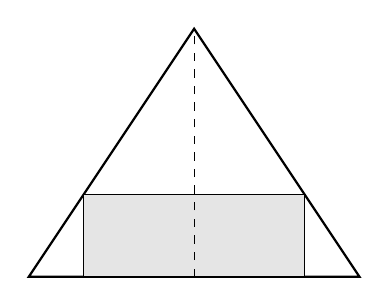
\begin{tikzpicture}[scale=0.7]
\draw[thick] (-3,0)--(0,4.5)--(3,0)--cycle;
\draw[fill=black!10] (-2,0) rectangle (2,1.5);
\draw[dashed] (0,0)--(0,4.5);
\end{tikzpicture}
\end{center}

\prob{u-tub}{The impossible tub}{after Q40, by John Newbold}
A tub is a frustum of a cone. Its larger end is 60\,cm across, and that is also the
diameter of a sphere passing through both rims. The cooper is asked to make it hold
50 litres. Can he?

\prob{u-ditch}{The shortest ditch}{after Q47, by John Edens of Tenerife}
A triangular field has sides of 200\,m, 150\,m and 60\,m. A straight ditch must divide it
into two equal areas. Where should it run so as to be as short as possible?

\prob{u-diamonds}{The diamond merchant}{after Q53, by Thomas Dodd}
A merchant sells sixteen diamonds whose prices form a geometric progression. The first
costs 1p and the last £143,489.07. What is the common ratio, and what do all sixteen cost
together?

\prob{u-walkers}{London and Norwich}{Q54, by Robert Beales of Lynn}
Two walkers set out at the same time from London and Norwich, 99 miles apart, to meet
each other. The Londoner walks 3 miles the first day, 5 the second, 7 the third, and so
on. The walker from Norwich covers, on the first day, a number of miles equal to
one-sixth of the number of days it takes them to meet, and 3 miles more each day after
that. When do they meet, and how far has each walked?

\prob{u-field}{The field that cannot exist}{after Q56, by W. Beriffe of St Ives}
A surveyor reports a four-sided field with sides of 40\,m, 60\,m, 70\,m and 50\,m in
order, and an area of 2,900\,m$^2$. Show that he must have made a mistake.

\prob{u-ellipse}{The elliptical tether}{after Q91, by Christopher Mason}
A horse is to graze exactly 1,000\,m$^2$ in the shape of an ellipse whose axes are in the
ratio $9:7$. It is tied to a loop of rope passed round two stakes, so that as it pulls
the rope taut it traces the ellipse. Where should the stakes go, and how long should the
loop be?
\begin{center}
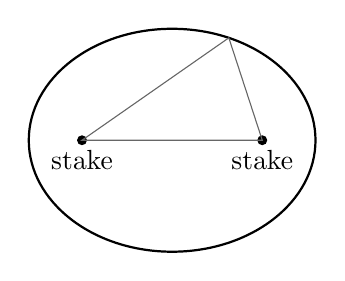
\begin{tikzpicture}[scale=0.09]
\draw[thick] (0,0) ellipse (20.23 and 15.73);
\fill (-12.72,0) circle (0.7) (12.72,0) circle (0.7);
\draw[black!60] (-12.72,0)--(8,14.45)--(12.72,0)--cycle;
\node[below] at (-12.72,0) {stake}; \node[below] at (12.72,0) {stake};
\end{tikzpicture}
\end{center}

\prob{u-series}{Two series for ever}{Q131, by Thomas Dodd}
Two geometric series are continued for ever. The sum of the first is to the sum of the
second as 4 to 9. The first two terms of the first series are 40 and 35, and the second
term of the second series is $46\tfrac{19}{36}$. Find the first term and the ratio of the
second series.

\prob{u-quad}{The largest quadrilateral}{Q134, by Thomas Grant}
Find the greatest area that can be enclosed by four straight lines of lengths 20, 16, 12
and 10.

\prob{u-circles}{Four circles in a triangle}{Q143, by Thomas Battersbye}
A circle is inscribed in a triangle. In each corner a small circle is drawn touching the two
sides and the large circle. The small circles have diameters 484, 441 and 400. Find the
diameter of the large circle and the sides of the triangle.
\begin{center}
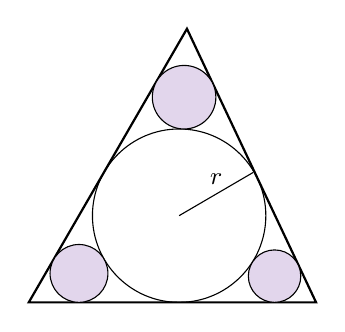
\begin{tikzpicture}[scale=1.5]
\coordinate (A) at (1.339,2.316); \coordinate (B) at (0,0); \coordinate (C) at (2.432,0);
\draw[thick] (A)--(B)--(C)--cycle;
\draw (1.273,0.734) circle (0.734);
\fill[bandpurple!20] (1.315,1.737) circle (0.269); \draw (1.315,1.737) circle (0.269);
\fill[bandpurple!20] (0.425,0.245) circle (0.245); \draw (0.425,0.245) circle (0.245);
\fill[bandpurple!20] (2.081,0.222) circle (0.222); \draw (2.081,0.222) circle (0.222);
\draw (1.273,0.734)--node[above]{\small $r$} (1.9,1.1);
\end{tikzpicture}
\end{center}

\prob{u-xx}{A number raised to itself}{Q146, by Thomas Grant}
Find $x$ such that $x^x = 123{,}456{,}789$, to six decimal places, by a method that works
for any number in place of $123{,}456{,}789$.

\prob{u-julian}{The year of her birth}{Q175, by Robert Fearnside}
Old almanacs gave three cycles for each year. For the year $N$: the solar cycle is the
remainder when $N+9$ is divided by 28; the golden number is the remainder when $N+1$ is
divided by 19; the indiction is the remainder when $N+3$ is divided by 15 (a remainder of
0 counts as 28, 19 or 15). A lady was born in a year whose solar cycle was 18, golden
number 8 and indiction 10. When was she born, and when will the same three numbers next
come round?

\prob{u-double}{Doubling money}{Q213, by Robert Heath}
At what rate of compound interest, $x$ per cent a year, will a sum of money double in
exactly $x$ years?

\prob{u-dice}{Four of a kind}{Q221, by Peter Kay}
A player undertakes, throwing six dice, to bring up four faces of the same kind (four
aces, four twos, and so on; five or six of a kind also count) in one of seven throws.
What are the odds against him?

\prob{u-grove}{The fountain in the grove}{Q260, by Nicholas Farrer}
In a triangular grove one side is 20\,m long and the angle opposite it is
$78^\circ45'$. The perpendiculars from the three corners to the opposite sides all meet
at a fountain, 8.19\,m from the given side. Find the other two sides.

\prob{u-fractions}{How many fractions?}{Q281, by John May of Amsterdam}
How many different fractions between 0 and 1 have a denominator less than 100? Fractions
of equal value, such as $\tfrac12$ and $\tfrac24$, count once.

\prob{u-courier}{The courier's crossing}{prize question, answered 1730}
A courier at Montpellier is ordered to Turin as fast as possible. The Rhone runs straight
from north to south between them. Montpellier is 40\,km west of the river, Turin 150\,km
east of it, and the two cities are 200\,km apart in a straight line. West of the river
the courier travels at 3\,km an hour, east of it only 2. Where should he cross the river?
\begin{center}
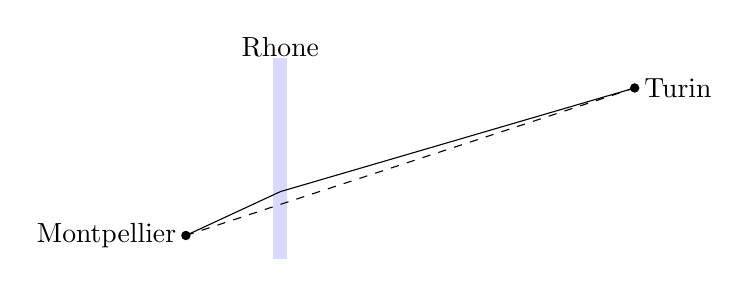
\begin{tikzpicture}[scale=0.03]
\fill[blue!15] (-3,-10) rectangle (3,75); \node at (0,80) {Rhone};
\fill (-40,0) circle (2) node[left]{Montpellier};
\fill (150,62.45) circle (2) node[right]{Turin};
\draw (-40,0)--(0,18.57)--(150,62.45);
\draw[dashed] (-40,0)--(150,62.45);
\end{tikzpicture}
\end{center}

\prob{u-chimney}{The pole in the chimney}{prize question, answered 1733, by Robert Fearnside}
A chimney opening runs back 1.2\,m from the front of the mantel to the back wall, and the
mantel is 2.4\,m above the hearth. What is the longest cylindrical pole, 30\,cm thick,
that can be got up the chimney?
% (b) The Diary also asks for the greatest conical pole that can be put up the same
% chimney, the slant side of the cone being to the diameter of its base as 4 to 1.
% Left out pending a decision; the Diary's answer is 14 ft 0.48 in (unchecked).
\begin{center}
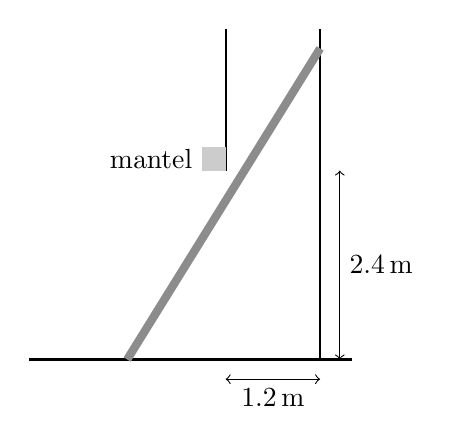
\begin{tikzpicture}[scale=1]
\draw[thick] (-2.5,0)--(1.6,0);
\draw[thick] (1.2,0)--(1.2,4.2);
\draw[thick] (0,2.4)--(0,4.2); \fill[black!20] (-0.3,2.4) rectangle (0,2.7);
\node[left] at (-0.3,2.55) {mantel};
\draw[line width=3pt,black!45] (-1.25,0)--(1.2,3.95);
\draw[<->] (0,-0.25)--(1.2,-0.25) node[midway,below]{1.2\,m};
\draw[<->] (1.45,0)--(1.45,2.4) node[midway,right]{2.4\,m};
\end{tikzpicture}
\end{center}

\prob{u-ceva}{Lines through a point}{prize question, answered 1736, by Samuel Ashby}
In any triangle $ABC$, lines from the three corners through a common point $O$ inside it
meet the opposite sides at $D$ (on $BC$), $E$ (on $CA$) and $F$ (on $AB$). Prove that
\[AF\cdot BD\cdot CE = FB\cdot DC\cdot EA.\]
\begin{center}
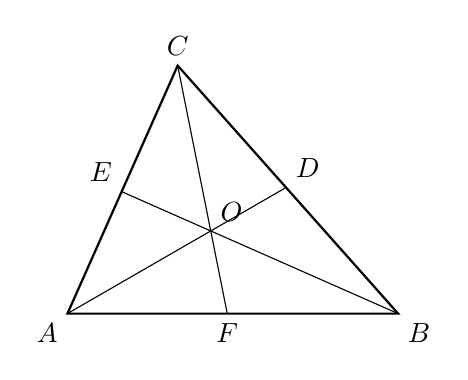
\begin{tikzpicture}[scale=0.7]
\coordinate (A) at (0,0); \coordinate (B) at (6,0); \coordinate (C) at (2,4.5);
\coordinate (O) at (2.6,1.5);
\draw[thick] (A)--(B)--(C)--cycle;
\coordinate (D) at (3.966,2.288); \coordinate (E) at (0.984,2.213); \coordinate (F) at (2.9,0);
\draw (A)--(D); \draw (B)--(E); \draw (C)--(F);
\node[above right] at (D) {$D$}; \node[above left] at (E) {$E$}; \node[below] at (F) {$F$};
\foreach \p/\l in {A/below left,B/below right,C/above,O/above right} \node[\l] at (\p) {$\p$};
\end{tikzpicture}
\end{center}
%================ ANSWERS ================
\clearpage
\section*{Answers}

\subsection*{\color{bandgreen}Green}
\ans{g1}{10 minutes.}
\ans{g2}{16 grains for the fifth box; $1+2+4+8+16 = 31$ altogether.}
\ans{g3}{Daughter 1, mother 2, son 4.}
\ans{g4}{6 days: ABC, ACB, BAC, BCA, CAB, CBA.}
\ans{g5}{Cat 8, dog 6, rabbit 4.}
\ans{g6}{Rows $4\,9\,2$; $3\,5\,7$; $8\,1\,6$.}

\subsection*{\color{bandblue}Blue}
\ans{b1}{A million million pounds at £100 a minute takes $10^{10}$ minutes. A year of
365 days 5 hours 45 minutes is 525,945 minutes, so the time is 19,013 years 144 days 5
hours 55 minutes.}
\ans{b2}{(a) 512. (b) 1, 3, 7, 15, 31: each total is one less than the grains on the next
diamond. (c) $2^{64}-1 = 18{,}446{,}744{,}073{,}709{,}551{,}615$ grains. A few sacks hold a
few million.}
\ans{b3}{The will makes the mother's share twice the daughter's and the son's twice the
mother's, so the shares go $1:2:4$: daughter £1,000, mother £2,000, son £4,000.}
\ans{b4}{$9\times8\times7\times\dots\times1 = 362{,}880$ days, about 993 years and 186
days.}
\ans{b5}{Add the three differences to the total and divide by four:
$(5219+22+73+130)/4 = 1361$. The votes are 1,361, 1,339, 1,288 and 1,231.}
\ans{b6}{One answer (the Diary's):
\begin{center}\begin{tabular}{cccc}
8&28&27&11\\ 23&15&16&20\\ 17&21&22&14\\ 26&10&9&29
\end{tabular}\end{center}}

\subsection*{\color{bandamber}Amber}
\ans{a-rhyme}{$x+\tfrac12x+\tfrac13x+9 = 130$, so $\tfrac{11}{6}x = 121$ and the age
is 66.}
\ans{a-wine}{£95 buys $5\times13 = 65$ barrels, which is 9,750 litres.}
\ans{a-hay}{90 loads cost $6\times£178 = £1{,}068$. The notes cover £320, so he needs 748
coins.}
\ans{a-wedding}{If the wife was $w$, then $3w+15 = 2(w+15)$, so $w = 15$. He was 45 and
she 15.}
\ans{a-coins}{The three pairs add up to $409 + 1254 + 1145 = 2808$, which counts every
coin twice, so there are 1,404 coins. Hence 995 £2 coins, 259 £1 coins and 150 50p
coins, worth £2,324.}
\ans{a-servant}{$16w = 20(27-w)$ gives $w = 15$: 15 days worked and 12 idle. (The
Diary's version gave the fractional answer 16 days 8 hours.)}
\ans{a-spark}{Working backwards: $4^2 = 16$; $16\div\tfrac29 = 72$; $72\div3 = 24$;
$24\div\tfrac27 = 84$; $84\div3 = 28$. She was 28.}
\ans{a-fisher}{The numbers are in the ratio $27:1$, so the less is
$16\tfrac12\div28 = \tfrac{33}{56}$ and the greater $\tfrac{891}{56} = 15\tfrac{51}{56}$.}
\ans{a-shepherd}{With $n$ shepherdesses there are $2n^2$ sheep, and $2^{n-1} = 2n^2$. By
trial $n = 8$: 8 shepherdesses and 128 sheep.}
\ans{a-months}{$\tfrac{13}{8}m = 442$, so $m = 272$ months: 22 years 8 months.}
\ans{a-brown}{$\left(1-\tfrac19+\tfrac13\right)x^2 = \tfrac{11}{9}x^2 = 891$, so
$x^2 = 729$ and she will be 27.}
\ans{a-army}{300 rows by 200 files. Between them are 299 and 199 gaps, so the ground is
$598\text{ m}\times398\text{ m} = 238{,}004\text{ m}^2$, about 23.8 hectares.}
\ans{a-estate}{$352947\times64\times9 = 203{,}297{,}472 = 588^3$. The estate is £588 and
the portion £252.}
\ans{a-names}{David, Lucia and Lidia. DAVID gives $D+V+I+D = 1006$, which is a thousand
more than U and I; LUCIA gives $50+5+100+1 = 156$; LIDIA gives $50+1+500+1 = 552$; and
$1006+156+552 = 1714$.}
\ans{a-walnut}{$3n^2 = 2187$, so $n^2 = 729$ and there were 27 trees.}
\ans{a-legacy}{$M:A = 3:2 = 15:10$ and $A:N = 5:4 = 10:8$, so $M:A:N = 15:10:8$. The
shares are £3,000, £2,000 and £1,600.}
\ans{a-magic10}{There are many answers. One is
\begin{center}\small\setlength{\tabcolsep}{4pt}\begin{tabular}{cccccccccc}
92 & 99 & 1 & 8 & 15 & 67 & 74 & 51 & 58 & 40\\
98 & 80 & 7 & 14 & 16 & 73 & 55 & 57 & 64 & 41\\
4 & 81 & 88 & 20 & 22 & 54 & 56 & 63 & 70 & 47\\
85 & 87 & 19 & 21 & 3 & 60 & 62 & 69 & 71 & 28\\
86 & 93 & 25 & 2 & 9 & 61 & 68 & 75 & 52 & 34\\
17 & 24 & 76 & 83 & 90 & 42 & 49 & 26 & 33 & 65\\
23 & 5 & 82 & 89 & 91 & 48 & 30 & 32 & 39 & 66\\
79 & 6 & 13 & 95 & 97 & 29 & 31 & 38 & 45 & 72\\
10 & 12 & 94 & 96 & 78 & 35 & 37 & 44 & 46 & 53\\
11 & 18 & 100 & 77 & 84 & 36 & 43 & 50 & 27 & 59\\
\end{tabular}\end{center}}
\ans{a-gold}{Multiplying the three products gives $(lbd)^2 = 921{,}600$, so the volume is
960\,cm$^3$. Dividing by each product: 12\,cm by 10\,cm by 8\,cm.}
\ans{a-lcm}{$2520 = 2^3\times3^2\times5\times7$. Rule: take each prime to the highest
power that appears in any of the given numbers, and multiply.}
\ans{a-world}{One circuit takes 450 days and the other 800. Both are home together after
the least common multiple, 7,200 days (about 19.7 years), when the first has gone round
16 times and the second 9.}
\ans{a-fares}{Exactly eight ways (captains, mates, sailors, boys): 1, 6, 15, 2;\quad
1, 7, 8, 8;\quad 1, 8, 1, 14;\quad 2, 4, 14, 4;\quad 2, 5, 7, 10;\quad 3, 2, 13, 6;\quad
3, 3, 6, 12;\quad 4, 1, 5, 14. The Diary printed only 2, 4, 14, 4 and remarked that the
question has ``innumerable answers''. It has eight.}
\ans{a-labourer}{$70w = 30(365-w)$ gives $w = 109\tfrac12$: $109\tfrac12$ days worked and
$255\tfrac12$ idle.}
\ans{a-aliquot}{20 and 33: the parts of 20 add to $1+2+4+5+10 = 22$, two-thirds of 33;
the parts of 33 add to $1+3+11 = 15$, three-quarters of 20. The proposer's own answer was
404 and 465, which also works.}
\ans{a-perfect}{If $2^n-1$ is prime, then $2^{n-1}(2^n-1)$ is perfect (Euclid, Book IX,
Proposition 36). Below ten million: 6, 28, 496, 8128. Euler later proved that every even
perfect number has this form. Nobody knows whether an odd one exists.}
\ans{a-field}{Multiplying out gives $3w + 2l = 58$ and $2w + 3l = 62$, so the field is
14\,m by 10\,m, with area 140\,m$^2$.}
\ans{a-battalion}{If the side is $n$, then $n^2+284 = (n+1)^2-25$, so $2n+1 = 309$ and
$n = 154$. There are $154^2+284 = 24{,}000$ soldiers.}
\ans{a-birthday}{The middle number cubed is 512, so it is 8, and the outer two multiply
to 64 and add to 34: they are 2 and 32. The age is 24 years 8 weeks, and the birthday is
2 August. (The Diary's solver dated it 2 August 1709.)}
\ans{a-billiards}{Reflect $B$ in the sixth cushion, reflect that image in the fifth, and
so on back to the first. The straight line from $A$ to the final image meets the first
cushion where $A$ must strike it. From that point, aim at the image made from the second
cushion onwards, and so on. Each reflection keeps the angles of bounce equal.}
\ans{a-clock}{The hands are opposite a little after seven, when
$6m - (210 + \tfrac12 m) = -180$ for $m$ minutes past, so $m = 5\tfrac{5}{11}$. The time
was $5\tfrac{5}{11}$ minutes past seven, with the line tilted about $57^\circ$.}

\subsection*{\color{bandpink}Pink}
\ans{p-garden}{If the width is $w$, then $w(100+80-w) = 4000$, so
$w = \tfrac12\left(180-\sqrt{16400}\right) \approx 25.97$\,m.}
\ans{p-fathers}{$x\cdot2x\cdot2x + 340\tfrac12 = 30000$ gives $x^3 = 7414.875$, so
$x = 19\tfrac12$. The men are 39 and the son $19\tfrac12$.}
\ans{p-vintner}{With $x$, $y$, $z$ bottles at £32, £20, £16: $z = 3x-28$ and $y = 84-4x$,
so every $x$ from 10 to 20 works. That is 11 ways.}
\ans{p-grind}{The circle left after $k$ shares have a diameter of $60\sqrt{(7-k)/7}$.
The seven people grind away 4.45, 4.84, 5.35, 6.08, 7.21, 9.39 and 22.68\,cm of the
diameter.}
\ans{p-tether}{$\sqrt{1000/\pi} \approx 17.84$\,m.}
\ans{p-kettle}{With diameters $5k$ and $3k$,
$V = \tfrac{\pi h}{12}\left(25+15+9\right)k^2 = 50{,}000$, which gives $k \approx 11.40$.
The diameters are about 57.0\,cm and 34.2\,cm.}
\ans{p-fractions}{$\tfrac1{11}$ and $\tfrac4{77}$.}
\ans{p-ship}{If $h$ is the direct distance, then $n\cdot w = 150h$ and $(w-n)^2 = h^2 -
300h$, which gives $h = 150+\sqrt{150^2+60^2} \approx 311.55$ miles. The ship sailed
188.25 miles north and 248.25 west, 436.50 in all.}
\ans{p-bushel}{$46\sqrt{20/18} \approx 48.5$\,cm.}
\ans{p-ladder}{$100-\sqrt{9900} \approx 0.50$\,m: only about 50\,cm.}
\ans{p-tippler}{$5x^{5/2} = 38{,}880$, so $x^{5/2} = 7776 = 6^5$ and $x = 36$: £36.}
\ans{p-maypole}{$63+\sqrt{63^2-30^2} = 63+\sqrt{3069} \approx 118.40$\,m.}
\ans{p-head}{The head travels on a circle 1.5\,m larger in radius, through the same
angle, $2\pi\times\tfrac{10000}{40000}$, so the extra distance is
$1.5\times\tfrac{\pi}{2} \approx 2.36$\,m. The size of the Earth does not matter, only the
fraction of the way round.}
\ans{p-ap}{15, 19, 23, 27.}
\ans{p-sons}{21 and 16.}
\ans{p-decagon}{A regular decagon of side $s$ has area $\tfrac52 s^2\sqrt{5+2\sqrt5}
\approx 7.694\,s^2$, so $s \approx 4.69$\,m.}
\ans{p-pond}{The radius is 40\,m. If $x$ is left standing, then $x^2+40^2 = (100-x)^2$,
so $x = 42$\,m.}
\ans{p-chords}{The radius is $(30^2+10^2)/(2\times10) = 50$\,m. The new height is
$50-\sqrt{50^2-45^2} \approx 28.21$\,m.}
\ans{p-field}{$\tfrac12\times16{,}000\times\sin30^\circ = 4{,}000$\,m$^2$.}
\ans{p-prize}{99 men, each getting £99, so £9,801 in all.}
\ans{p-earth}{The radius is $40{,}000/2\pi \approx 6366$\,km, so the volume is about
$1.08\times10^{21}$\,m$^3$. The river brings $72{,}000$\,m$^3$ an hour, so it takes
about $1.7\times10^{12}$ years. The Diary, with its own figures, found about
$2.3\times10^{12}$.}
\ans{p-house}{Cost £250, profit £90.}
\ans{p-temples}{38\,m and 26\,m.}
\ans{p-extreme}{The shares divide £50,000 in extreme and mean ratio:
$50{,}000\times\tfrac{\sqrt5-1}{2} \approx £30{,}901.70$ to the elder and £19,098.30 to the
younger.}
\ans{p-tub}{By similar triangles the top is $32\times\tfrac{30}{20} = 48$\,cm across, and
the depth is 30\,cm. The volume is
$\tfrac{\pi\times30}{12}(48^2+48\times32+32^2) = 12{,}160\pi \approx 38{,}200$\,cm$^3$,
about 38.2 litres.}
\ans{p-southsea}{A £17,000, B £15,000, C £8,000.}
\ans{p-moat}{About 151.27\,m (the ladder is about 177.57\,m).}
\ans{p-golden}{The breadth, length and diagonal are in the ratio $1:\sqrt\varphi:\varphi$,
where $\varphi = \tfrac{1+\sqrt5}{2}$. The sides are about 129.8\,m and 165.1\,m, with a
diagonal of 210.1\,m. The area is about 21,440\,m$^2$, which costs about £42,880.}
\ans{p-quotients}{About 8,273.27 and 1,726.73.}
\ans{p-close}{The segments of the diagonal are 16\,m and 4\,m, so the diagonal is
20\,m and the perpendicular $\sqrt{16\times4} = 8$\,m. The field is $8\sqrt5$ by
$4\sqrt5$, about 17.89\,m by 8.94\,m. The four shares are 64, 16, 4 and 76\,m$^2$,
totalling 160\,m$^2$.}
\ans{p-molten}{The outside diameter is $30\times55.6/\pi \approx 531$\,cm and the inside
$\approx 512.3$\,cm; the depth is 278\,cm. So a bath is about 28.7 litres.}
\ans{p-york}{Stilton is $150\times\tfrac{3-\sqrt5}{2} \approx 57.3$ miles from London. The
speeds are in the ratio $0.382:1$, so the York messenger goes $\varphi^2 \approx 2.618$
times as fast.}
\ans{p-eclipse}{The base satisfies $b^2+66b-6567 = 0$, so the sides are about 54.50,
28.50 and 61.50.}
\ans{p-speidel}{Put $C$ at the origin with $CA$ along the axis, $CA = a$ and $BP = h$. The
bisector is $y = x$, and $DA$ is $y = h - \tfrac{h}{a}x$, so they meet at $N = (s,s)$ with
$s = \tfrac{ah}{a+h}$. At height $s$ the triangle is $a\left(1-\tfrac{s}{h}\right) =
\tfrac{ah}{a+h} = s$ wide. So $GH$ equals its own height above $CA$: it is the top of the
square.}
\ans{p-legs}{With $AB = a$ and $BC = c$, similar triangles give
$BF = BG = \tfrac{ac}{a+c}$, $AF = \tfrac{a^2}{a+c}$ and $CG = \tfrac{c^2}{a+c}$, so
$AF\cdot CG = BF^2$.}
\ans{p-steeple}{The area $\tfrac12 xy\sin\theta$ is largest at $\theta = 90^\circ$, and
the third side $\sqrt{x^2+y^2}$ is then least when $x = y$. It is $\sqrt{2\times1800} =
60$\,m.}
\ans{p-manors}{192, 384, 768 and 1,536 hectares.}
\ans{p-stone}{12\,cm, 18\,cm and 24\,cm.}
\ans{p-pigs}{A husband and wife who buy $h$ and $w$ pigs satisfy $h^2 - w^2 = 63$, so the
pairs are 32 and 31, 12 and 9, or 8 and 1. Hendrick is married to Anna (32 and 31),
Claas to Catriin (12 and 9), and Cornelius to Geertruii (8 and 1).}
\ans{p-firs}{The fountain is 75\,m from the foot of the shorter fir and 45\,m from the
taller. The balls are $\sqrt{120^2+20^2} \approx 121.66$\,m apart. The walk runs at right
angles to the line of the trees, and the summer-house is 91.65\,m from the foot of the
shorter fir and 69.28\,m from the taller. The walk is about 52.68\,m long.}

\begin{diarynote}{The grindstone and the lecturer}
Charles Hutton gave the neat construction for problem~\ref{p-grind} around 1770, while
the travelling lecturer James Ferguson was staying with him in Newcastle. Ferguson could
not follow the proof, so he drew the figure on a large sheet of pasteboard and measured
it. It agreed ``to a hair's breadth'', and he called it a treasure. (Leybourn, vol.~I,
pp.~7--8.)
\end{diarynote}

\subsection*{\color{bandpurple}Purple}
\ans{u-tokens}{$43x + 34y = 40{,}000$ has the solutions $x = 34n-2$, $y = 1179-43n$ for
$n = 1,\dots,27$. That is 27 ways, from 32 and 1,136 tokens up to 916 and 18.}
\ans{u-general}{$\binom{100}{10} = 17{,}310{,}309{,}456{,}440$ pennies, about £173
billion.}
\ans{u-sidway}{Cut the cone at one-third of its height. The cylinder has two-thirds of
the base radius and $\tfrac49$ of the cone's volume.}
\ans{u-tub}{No. With a sphere of radius 30\,cm, the volume is greatest when the smaller
diameter is about $0.647\times60 \approx 38.8$\,cm, and it is then only about 44.5
litres.}
\ans{u-ditch}{The shortest dividing line cuts off an isosceles triangle at the corner
with the smallest angle, between the 200\,m and 150\,m sides. It meets each of those sides
$\sqrt{15{,}000} \approx 122.5$\,m from that corner, and the ditch is about 23.45\,m
long.}
\ans{u-diamonds}{$3^{15} = 14{,}348{,}907$, so the ratio is 3. The total is
$(3^{16}-1)/2 = 21{,}523{,}360$p, which is £215,233.60.}
\ans{u-walkers}{They meet after 6 days. The Londoner walks $3+5+\dots+13 = 48$ miles, and
the other $1+4+\dots+16 = 51$.}
\ans{u-field}{By Brahmagupta's formula the largest area is
$\sqrt{(s-a)(s-b)(s-c)(s-d)}$ with $s = 110$, which is $\sqrt{70\times50\times40\times60}
\approx 2{,}898$\,m$^2$. That is just below 2,900.}
\ans{u-ellipse}{The axes are about 40.46\,m and 31.47\,m. The stakes go at the foci,
$\sqrt{a^2-b^2}$ from the centre, so about 25.43\,m apart. The loop is the major axis plus
that distance, about 65.89\,m.}
\ans{u-series}{The first sum is $40/(1-\tfrac78) = 320$, so the second is 720. From
$ar = 46\tfrac{19}{36}$ and $a/(1-r) = 720$ we get $a^2 - 720a + 33{,}500 = 0$. Either
$a = 50$ and $r = \tfrac{67}{72}$, or $a = 670$ and $r = \tfrac{5}{72}$.}
\ans{u-quad}{The largest quadrilateral is the one that can be inscribed in a circle. Its
area is $\sqrt{9\times13\times17\times19} = \sqrt{37{,}791} \approx 194.40$.}
\ans{u-circles}{The large circle has diameter 1,322. A small circle and the large one sit in the
same corner, so if the corner's angle is $A$ and the radii are $a$ and $r$,
$\sin\tfrac A2 = \tfrac{r-a}{r+a}$, which gives $\tan\tfrac A2 = \tfrac{r-a}{2\sqrt{ar}}$. The three
half-angles add up to $90^\circ$, and working this through gives
$r = \sqrt{ab} + \sqrt{bc} + \sqrt{ca}$. Battersbye chose his circles so that every product
is a square: with radii 242, $220\tfrac12$ and 200, $r = 231 + 210 + 220 = 661$. The sides
follow from the tangent lengths $r/\tan\tfrac A2$: about 2,407.7, 2,188.4 and 2,304.6.
Richard Lovet's printed sides differ only in the last places.

\emph{Another way, with complex numbers.} The relation above can be written
$\tan\tfrac A2 = \cot 2\phi_A$, where $\tan\phi_A = \sqrt{a/r}$, so $\tfrac A2 = 90^\circ - 2\phi_A$.
Adding over the three corners gives $\phi_A + \phi_B + \phi_C = 90^\circ$. The number
$\sqrt r + i\sqrt a$ has argument $\phi_A$, and so on, so the product
$(\sqrt r + i\sqrt a)(\sqrt r + i\sqrt b)(\sqrt r + i\sqrt c)$ is purely imaginary. Its real
part, $r\sqrt r - \sqrt r\,(\sqrt{ab} + \sqrt{bc} + \sqrt{ca})$, is therefore zero, and
$r = \sqrt{ab} + \sqrt{bc} + \sqrt{ca}$ follows at once.}

\ans{u-xx}{Solve $x\ln x = \ln123{,}456{,}789$ by Newton's method: $x \approx 8.640026$.}
\ans{u-julian}{We need $N \equiv 9 \pmod{28}$, $N \equiv 7 \pmod{19}$ and $N \equiv 7
\pmod{15}$, which gives $N = 1717$. The three repeat together every $28\times19\times15 =
7980$ years (the Julian period), so next in 9697.}
\ans{u-double}{Solve $x\ln\!\left(1+\tfrac{x}{100}\right) = \ln2$: $x \approx 8.498$ per
cent.}
\ans{u-dice}{One throw succeeds in $6\left[\binom64 5^2+\binom65 5+1\right] = 2436$ of
the 46,656 cases, so with probability about 0.0522. In seven throws the chance of at
least one success is $1-(1-0.0522)^7 \approx 0.313$. The odds are about 2.2 to 1 against
him.}
\ans{u-grove}{The circumradius is $R = 20/(2\sin78^\circ45') \approx 10.20$. The
fountain, the orthocentre, is $2R\cos B\cos C$ from the given side, so
$\cos B\cos C \approx 0.4016$ with $B + C = 101^\circ15'$. This gives $B \approx 52.3^\circ$
and $C \approx 49.0^\circ$, and the other sides are about 16.13\,m and 15.38\,m.}
\ans{u-fractions}{For each denominator $n$ from 2 to 99 there are $\varphi(n)$ fractions in
lowest terms, and $\sum_{n=2}^{99}\varphi(n) = 3003$.}
\ans{u-courier}{He should cross about 18.57\,km from the point due east of Montpellier,
on Turin's side. That gives 44.10\,km before the river and 156.29\,km after, taking about
92.8 hours. At the best crossing, $\sin\theta_1/3 = \sin\theta_2/2$, where the angles are
measured from the perpendicular to the river: the law of refraction.}
\ans{u-chimney}{About 4.37\,m. In the Diary's feet (a mantel 8\,ft high, an opening 4\,ft
deep and a pole 1\,ft thick) the answer is 14\,ft 7.2\,in.}
\ans{u-ceva}{Triangles with the same height have areas in proportion to their bases, so
$\tfrac{AF}{FB} = \tfrac{[AOC]}{[BOC]}$, $\tfrac{BD}{DC} = \tfrac{[AOB]}{[AOC]}$ and
$\tfrac{CE}{EA} = \tfrac{[BOC]}{[AOB]}$. Multiplying, the product is 1. This is Ceva's
theorem, published in 1678.}

\begin{diarynote}{When the Diary was wrong}
\textbf{Problem~\ref{u-field}.} The original surveyor's figures (sides 4, 6, 7 and 5
chains, area 29 square chains) also exceed the largest possible area, $\sqrt{840}\approx
28.98$. The first solver found a diagonal anyway. Leybourn's edition points out that
``the original solution cannot therefore be correct''.

\textbf{Problem~\ref{u-series}.} The Diary gave only the first answer, 50 and
$\tfrac{67}{72}$. The quadratic has a second root, 670 and $\tfrac5{72}$, which fits every
condition just as well.

\textbf{Problem~\ref{u-grove}.} The printed solution assumed the triangle was isosceles,
with two equal sides of 15.64. It is not; the later editor showed that the sides differ.

\textbf{Problem~\ref{u-walkers}.} The Diary's answer swaps the walkers, crediting the
Norwich walker with 48 miles and the Londoner with 51.

\textbf{Problem~\ref{u-fractions}.} One solver set out a method but gave no total;
another reached 3,055 and doubted it. The right answer is 3,003.

\textbf{Problem~\ref{a-fares}.} ``Innumerable answers'', said the Diary. There are
exactly eight.
\end{diarynote}

\end{document}
